\chapter{Pruebas y Validación}
\label{cap:pruebasValidacion}

\chapterquote{El primer principio es que no debes engañarte a ti mismo, y tú eres la persona más fácil de engañar.}{Richard Feynman}

Este capítulo recoge la validación del sistema desde dos perspectivas complementarias.
La primera, de carácter funcional, comprueba que el motor de exploración se comporta
correctamente sobre los dos dominios de prueba seleccionados (TMDB y DBLP) y se aborda
brevemente en la sección~\ref{sec:validacionFuncional}, ya que las decisiones técnicas
correspondientes se han descrito en el capítulo~\ref{cap:desarrolloImplementacion}. La
segunda, que ocupa el grueso del capítulo, es una evaluación formal de usabilidad con
participantes externos, presentada en la sección~\ref{sec:evalUsabilidad} y desarrollada
en las secciones~\ref{sec:resultadosCuantitativos} (resultados cuantitativos),
\ref{sec:hallazgosCualitativos} (hallazgos cualitativos),
\ref{sec:iteracionesUI} (iteraciones de interfaz derivadas) y
\ref{sec:casosDeUsoValidados} (casos de uso validados). La sección~\ref{sec:limitacionesEstudio}
cierra el capítulo reconociendo de manera explícita los límites del estudio.

\section{Validación funcional sobre TMDB y DBLP}
\label{sec:validacionFuncional}

La validación funcional del motor se ha realizado de manera incremental durante el desarrollo,
sobre dos volcados de catálogos públicos de naturaleza estructural muy distinta: TMDB
(\textit{The Movie Database}), que reúne películas, series y personas con metadatos descriptivos
y relaciones de participación, y DBLP, una base bibliográfica que reúne publicaciones
científicas, autores y lugares de publicación. La elección deliberada de dos dominios separados
ha permitido comprobar empíricamente que las primitivas del motor (filtrado facetado, navegación
transversal mediante \textit{links} y operaciones de conjunto) generalizan sin necesidad de
modificaciones sustanciales del modelo relacional, y constituye uno de los argumentos centrales
del trabajo. Las decisiones de diseño y los obstáculos encontrados durante esta integración se
detallan en el capítulo~\ref{cap:desarrolloImplementacion}; en lo que sigue se aporta evidencia
visual de la equivalencia operativa de ambos dominios.

La equivalencia entre ambos dominios se manifiesta ya en las pantallas previas a la navegación.
La figura~\ref{fig:seleccionDataset} muestra la primera pantalla del sistema, donde se ofrecen
los dos datasets disponibles. La lista se construye dinámicamente a partir de la tabla
\texttt{datasets} de PostgreSQL, de manera que añadir un nuevo dominio sólo requiere extender
los datos, no la interfaz. Una vez elegido uno, la pantalla siguiente expone las colecciones
publicadas por ese dataset (figura~\ref{fig:seleccionColecciones}): la disposición, tipografía
y controles son idénticos en ambos casos, lo que cambia es únicamente el conjunto de colecciones
ofrecidas, que proviene de la tabla \texttt{collections} poblada por los pipelines de ingesta
descritos en el Apéndice~\ref{Appendix:integracion}.

\begin{figure}[H]
\centering
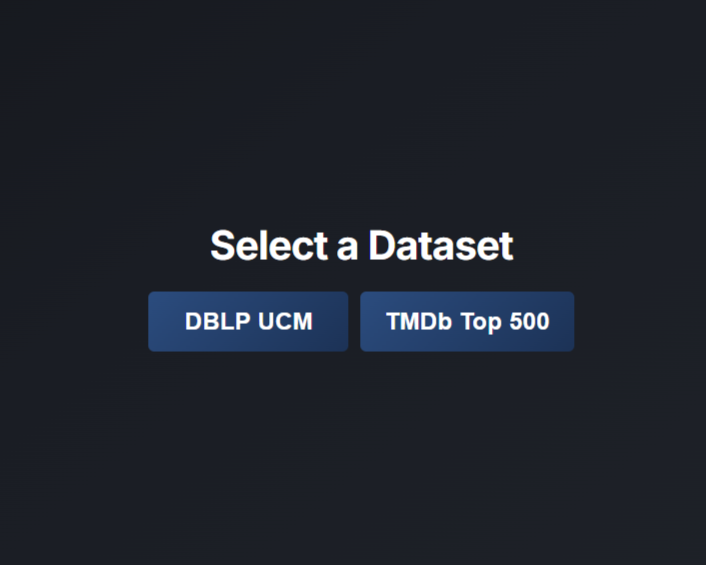
\includegraphics[width=0.45\textwidth]{Imagenes/Bitmap/validacion/seleccion_dataset.png}
\caption[Pantalla de selección de \textit{Dataset}]{Pantalla de entrada: selección de \textit{Dataset}.}
\label{fig:seleccionDataset}
\end{figure}

\begin{figure}[H]
\centering
\subfloat[][Colecciones expuestas por TMDB.]{%
  
\includegraphics[width=0.45\textwidth]{Imagenes/Bitmap/validacion/seleccion_colecciones_tmdb.png}
  \label{fig:coleccionesTMDB}}%
\qquad
\subfloat[][Colecciones expuestas por DBLP.]{%
  
\includegraphics[width=0.45\textwidth]{Imagenes/Bitmap/validacion/seleccion_colecciones_dblp.png}
  \label{fig:coleccionesDBLP}}
\caption[Selección de colección tras escoger \textit{Dataset}]{Selección de \textit{Collection} en cada uno de los dos dominios.}
\label{fig:seleccionColecciones}
\end{figure}

Una vez dentro de la vista de navegación se hace patente la equivalencia operativa del motor.
La figura~\ref{fig:dosDominios} muestra dos estados análogos: en TMDB, la colección
\textit{Movies} restringida por el filtro de metadatos \textit{Genre = Drama}; en DBLP, la
colección \textit{Publications} restringida por el filtro \textit{NumberOfCreators} en el rango
\textit{5--9}. Ambas vistas exhiben los mismos paneles (Filtros, \textit{Filtered Collection},
\textit{Links}, \textit{Union Set}) en las mismas posiciones, e idénticos controles de filtrado
e inclusión\,/\,exclusión; lo único que cambia es el contenido, producto de cargar un
\textit{Dataset} distinto sin modificar ni el esquema relacional ni la lógica del motor. La
transversalidad del modelo de \textit{links} se demuestra de manera análoga: pulsar sobre
\textit{Persons} en TMDB o sobre \textit{Authors} en DBLP produce el mismo tipo de navegación,
sin que el motor sepa que pasa de películas a artículos científicos.

\begin{figure}[H]
\centering
\subfloat[][TMDB: \textit{Movies} filtradas por \textit{Genre = Drama}.]{%
  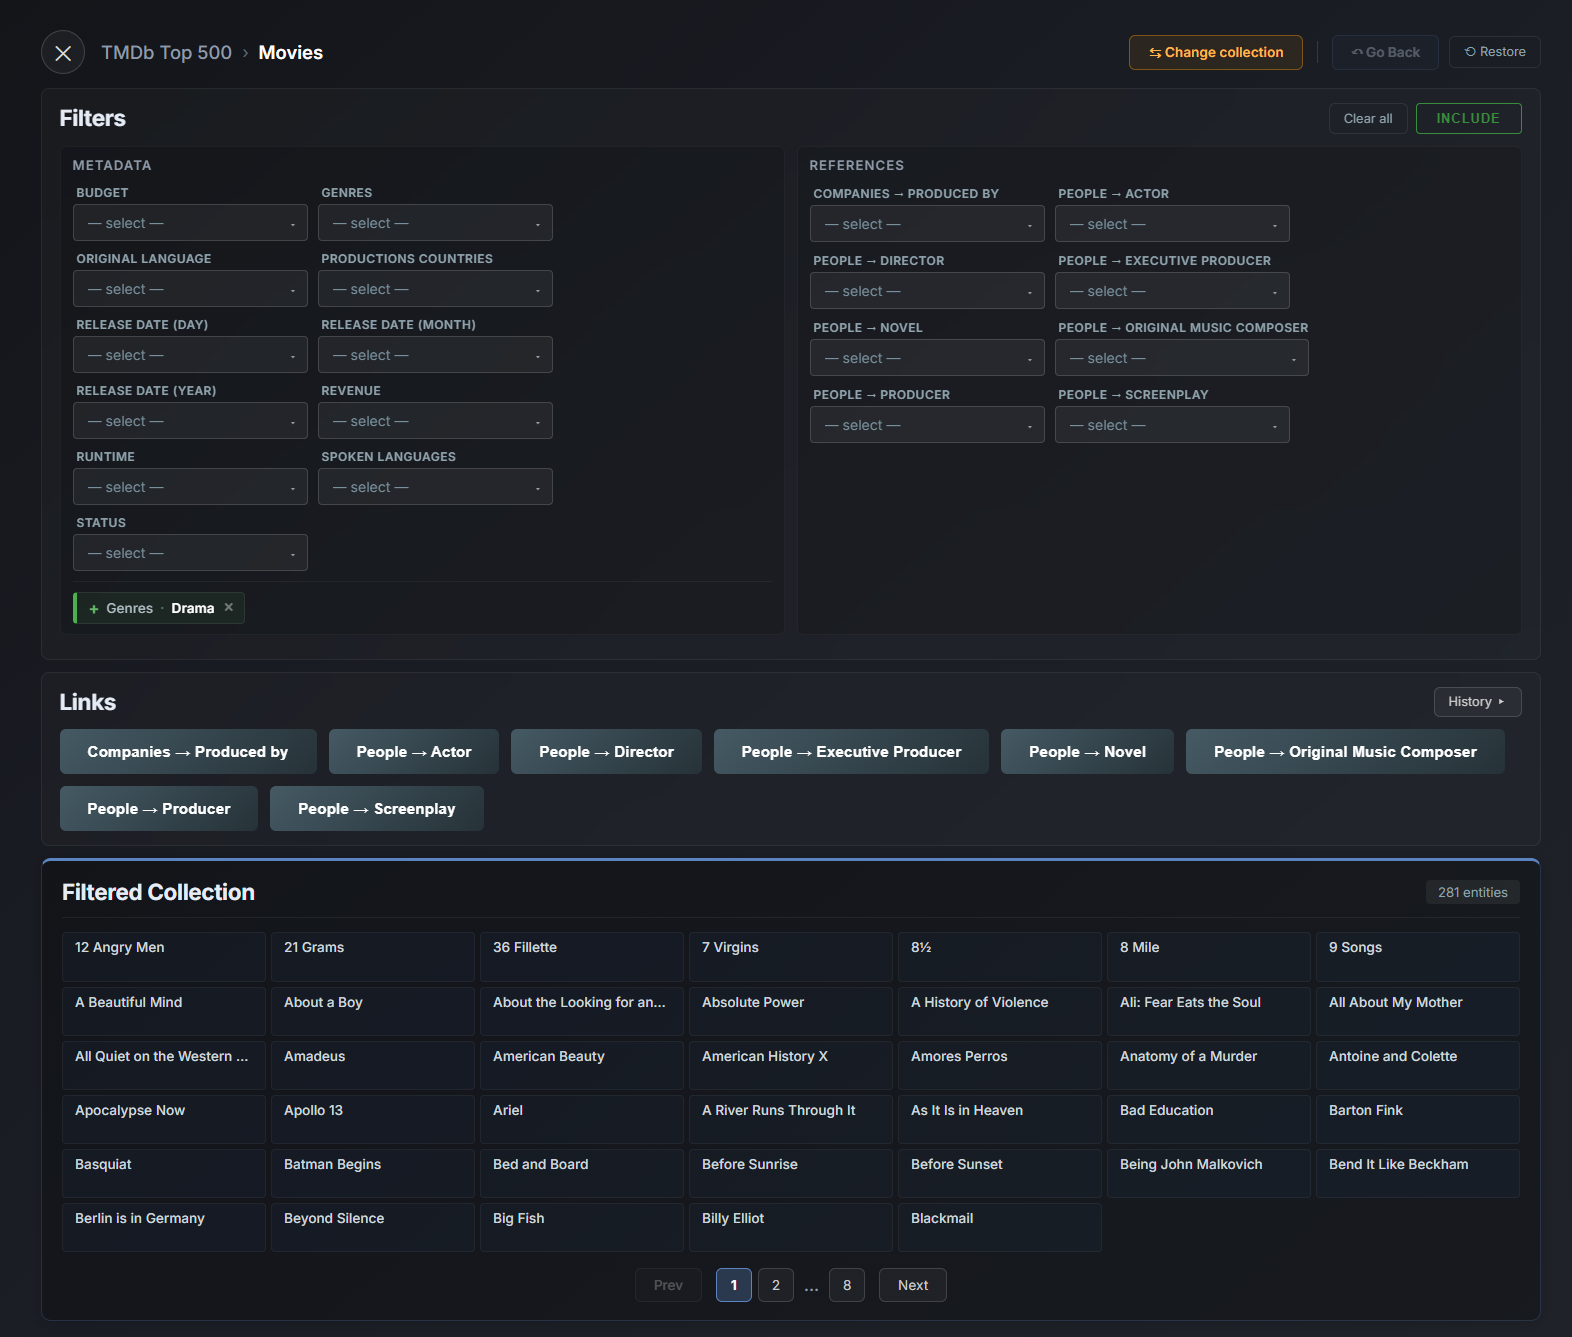
\includegraphics[width=0.95\textwidth]{Imagenes/Bitmap/validacion/tmdb_movies_drama.png}
  \label{fig:dominioTMDB}}\\[0.6em]
\subfloat[][DBLP: \textit{Publications} filtradas por \textit{NumberOfCreators = 5--9}.]{%
  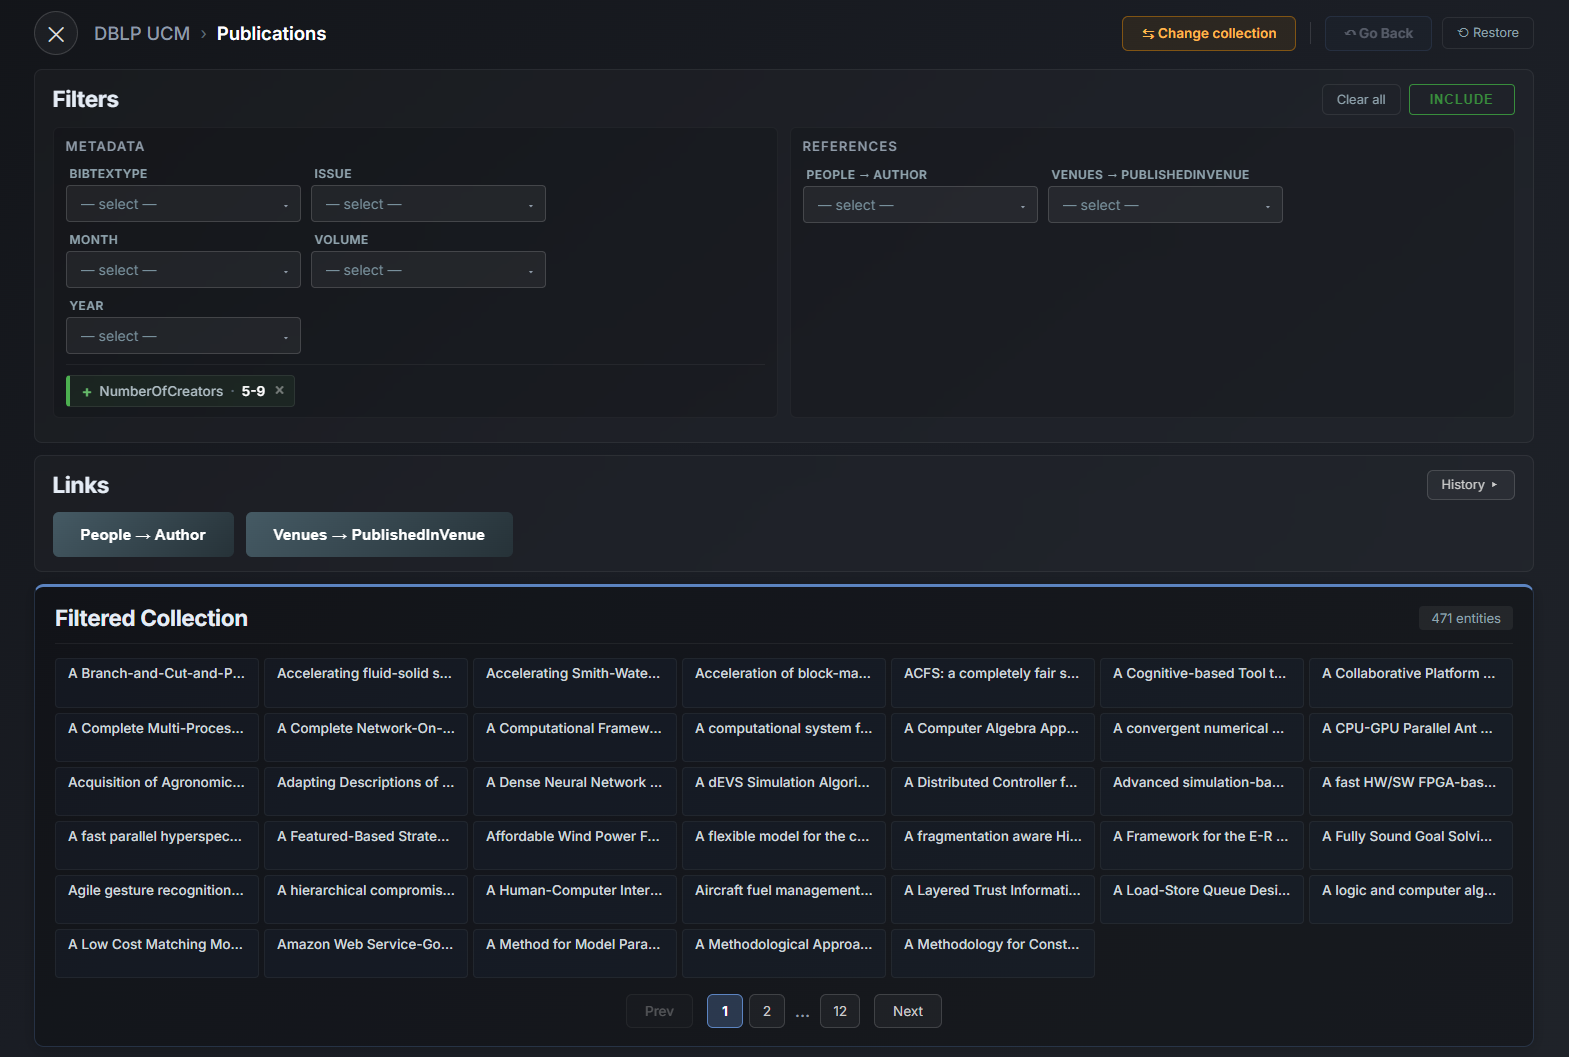
\includegraphics[width=0.95\textwidth]{Imagenes/Bitmap/validacion/dblp_publications_creators.png}
  \label{fig:dominioDBLP}}
\caption[Misma interfaz aplicada a TMDB y DBLP]{Estado análogo del motor de exploración sobre ambos dominios.}
\label{fig:dosDominios}
\end{figure}

La equivalencia se extiende también a la vista de inspección. La figura~\ref{fig:dosDetalles}
recoge el modal de detalle abierto sobre una entidad de cada dominio: una película de TMDB y una
publicación de DBLP. La estructura del modal y la manera de presentar los metadatos son
idénticas; los campos mostrados se obtienen de la tabla \texttt{metadata} para la entidad
concreta, sin que el \textit{frontend} conozca el dominio, lo que permite que el mismo
componente sirva para cualquier dataset sin código específico.

\begin{figure}[H]
\centering
\subfloat[][Detalle de una película (TMDB).]{%
  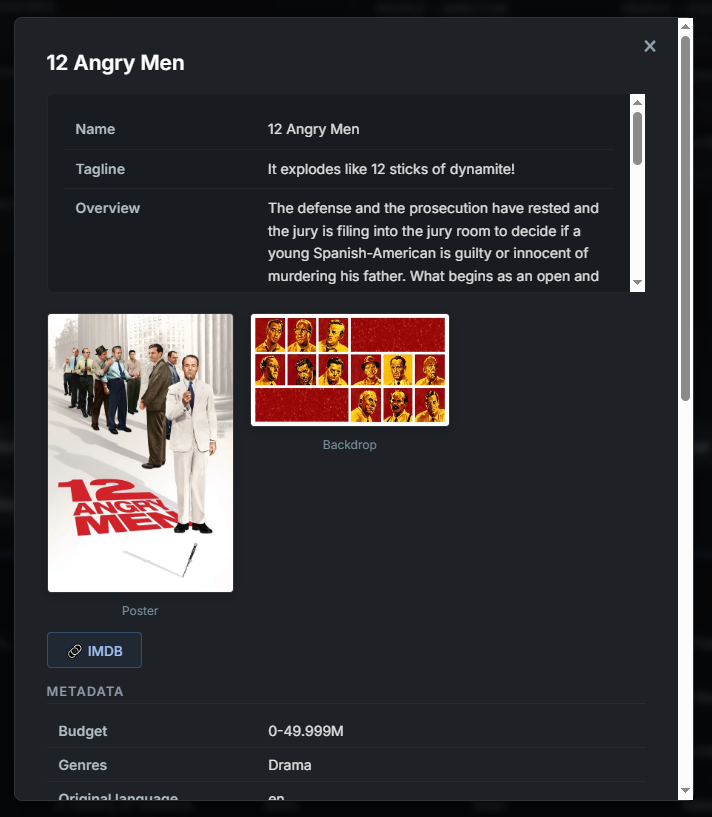
\includegraphics[width=0.45\textwidth]{Imagenes/Bitmap/validacion/tmdb_detalle_pelicula.png}
  \label{fig:detalleTMDB}}%
\qquad
\subfloat[][Detalle de una publicación (DBLP).]{%
  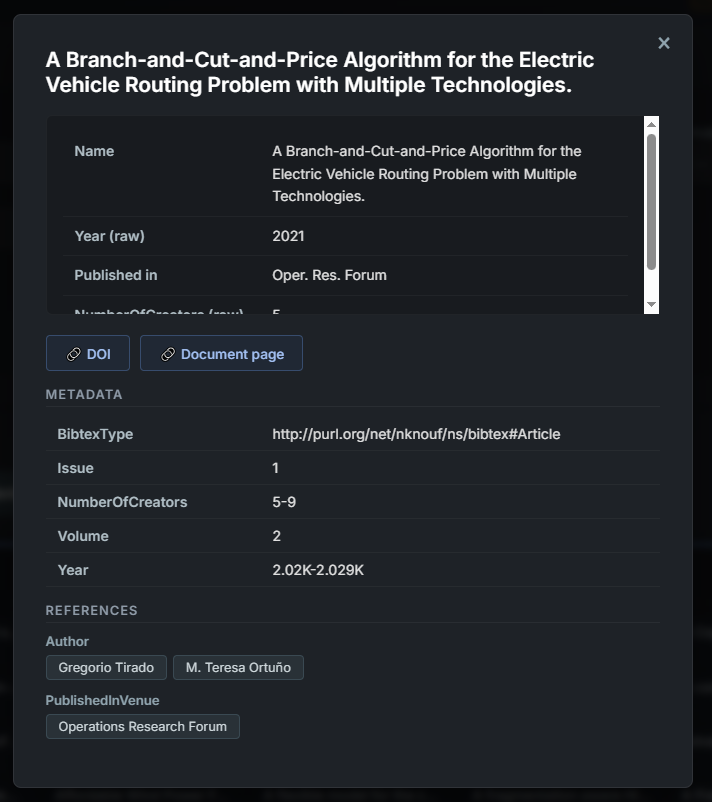
\includegraphics[width=0.45\textwidth]{Imagenes/Bitmap/validacion/dblp_detalle_publicacion.png}
  \label{fig:detalleDBLP}}
\caption[Modal de detalle aplicado a TMDB y DBLP]{Modal de detalle de una entidad sobre cada dominio.}
\label{fig:dosDetalles}
\end{figure}

La conclusión de esta validación funcional es que el motor cumple su pretensión de
generalidad: los mismos paneles, controles y operaciones funcionan sobre dos dominios de
estructura y temática muy distintas sin necesidad de tocar ni el esquema relacional ni el
código del motor. La evaluación con usuarios que ocupa el resto del capítulo se desarrolla,
por razones de familiaridad del participante, exclusivamente sobre TMDB; los hallazgos de
usabilidad recogidos a continuación son, en su mayoría, independientes del dominio concreto
sobre el que se navegue.

\section{Evaluación de usabilidad con usuarios}
\label{sec:evalUsabilidad}

\subsection{Objetivos del estudio}

La evaluación se diseñó con cinco objetivos explícitos que guían tanto el diseño del estudio
como la lectura posterior de los resultados:

\begin{itemize}
\item \textbf{Facilidad de aprendizaje} en la primera toma de contacto con el sistema, sin
formación ni documentación previa.

\item \textbf{Eficiencia} al realizar tareas comunes de búsqueda y navegación, medida en
tiempo y en cantidad de asistencia requerida.

\item \textbf{Comprensión de los conceptos clave} sobre los que se asienta el modelo de
navegación: filtros de inclusión y exclusión, \textit{links} entre colecciones, conjunto
unión, historial visual y la distinción entre \textit{Restore} y \textit{Go Back}.

\item \textbf{Recuperación ante errores} y manejo correcto de las acciones destructivas
(\textit{Exit} y \textit{Change collection}), que reinician parte del estado de la sesión.

\item \textbf{Satisfacción subjetiva}, recogida mediante el cuestionario estandarizado SUS
(\textit{System Usability Scale}) y un bloque de preguntas abiertas de cierre.
\end{itemize}

\subsection{Metodología}

El estudio sigue un protocolo formal de \textit{think-aloud} acompañado de observación
directa y de cuestionarios pre y post sesión. Cada participante realiza, en orden fijo,
catorce tareas planteadas como escenarios realistas, sin instrucciones procedimentales:
se enuncia el objetivo y el participante decide cómo resolverlo. Durante cada tarea, el
facilitador anota tiempo, completitud (\textit{Éxito} / \textit{Parcial} / \textit{Fallo}),
fluidez de navegación, estrategia seguida, nivel de asistencia requerido y satisfacción
aparente. Tras cada tarea se recoge la métrica \textbf{SEQ} (\textit{Single Ease Question},
escala de 1 a 7) y un comentario abierto. Al final de la sesión se administra el cuestionario
\textbf{SUS} (diez ítems en escala Likert de 1 a 5, con la fórmula clásica de cálculo que
produce una puntuación entre 0 y 100) y un bloque de ocho preguntas abiertas que recogen
percepciones globales y propuestas de mejora. El guion completo del estudio, incluyendo
texto literal a leer, hojas de consentimiento, plantillas de observación y notas
metodológicas, se reproduce íntegro en el Apéndice~\ref{Appendix:Guion}.

Cada sesión tuvo una duración aproximada de entre 32 y 37 minutos, con media en torno a
34~minutos, en línea con la estimación previa de 35-45~minutos. Las sesiones se realizaron
de manera presencial entre el 7 y el 14 de mayo de 2026, sobre la misma versión del sistema
y la misma colección inicial para asegurar comparabilidad. Cuatro de las cinco sesiones
fueron grabadas con permiso explícito del participante, y las grabaciones se eliminaron
una vez codificadas las observaciones.

\subsection{Perfil de los participantes}

Se reclutaron cinco participantes con perfiles diversificados, siguiendo la recomendación de
Nielsen según la cual cinco evaluadores descubren aproximadamente el 85\% de los problemas
de usabilidad observables en un sistema. La diversidad demográfica y disciplinar buscada
quedó representada como muestra el cuadro~\ref{tab:perfilParticipantes}: tres rangos de
edad distintos, cinco ocupaciones diferentes, dos personas con experiencia en catalogación
o bases de datos y tres sin ella, y una distribución equilibrada de la comodidad
auto-percibida con herramientas digitales nuevas (rango de 2 a 5 sobre 5).

\begin{table}[H]
\centering
\small
\begin{tabularx}{\textwidth}{c c X c c}
\hline
\textbf{ID} & \textbf{Edad} & \textbf{Ocupación} & \textbf{Catalogación} & \textbf{Comodidad} \\
\hline
P01 & 18--24 & Estudiante de Derecho y Filosofía & No                  & 3 \\
P02 & 18--24 & Estudiante de Ingeniería Informática & Sí (en estudios) & 5 \\
P03 & 25--34 & Médico                          & No                       & 2 \\
P04 & 18--24 & Programador                     & Sí (profesional)         & 4 \\
P05 & 55+    & Profesional administrativo      & No                       & 3 \\
\hline
\end{tabularx}
\caption[Perfil demográfico de los participantes]{Perfil demográfico y de experiencia previa de los cinco participantes. La columna
\textit{Comodidad} recoge la respuesta a la pregunta sobre comodidad para aprender una
herramienta nueva por cuenta propia, en escala de 1 a 5.}
\label{tab:perfilParticipantes}
\end{table}

\section{Resultados cuantitativos}
\label{sec:resultadosCuantitativos}

\subsection{Tasa de éxito y completitud}

De las setenta tareas realizadas en total (catorce tareas $\times$ cinco participantes),
sesenta y cinco se completaron con éxito sin asistencia y dentro del tiempo límite, lo que
arroja una tasa global de éxito del \textbf{93\%}. Las cinco situaciones restantes se reparten
entre dos parciales (T4 y T12 en P01, ambas resueltas con asistencia ligera) y dos fallos
(T2 en P03, derivado de una mala interpretación inicial de la tarea y no de la interfaz; y
T4 en P05, donde el participante no consiguió cambiar al modo de exclusión). El
gráfico~\ref{fig:tasaExitoTareas} desglosa estas categorías por tarea.

\begin{figure}[H]
\centering
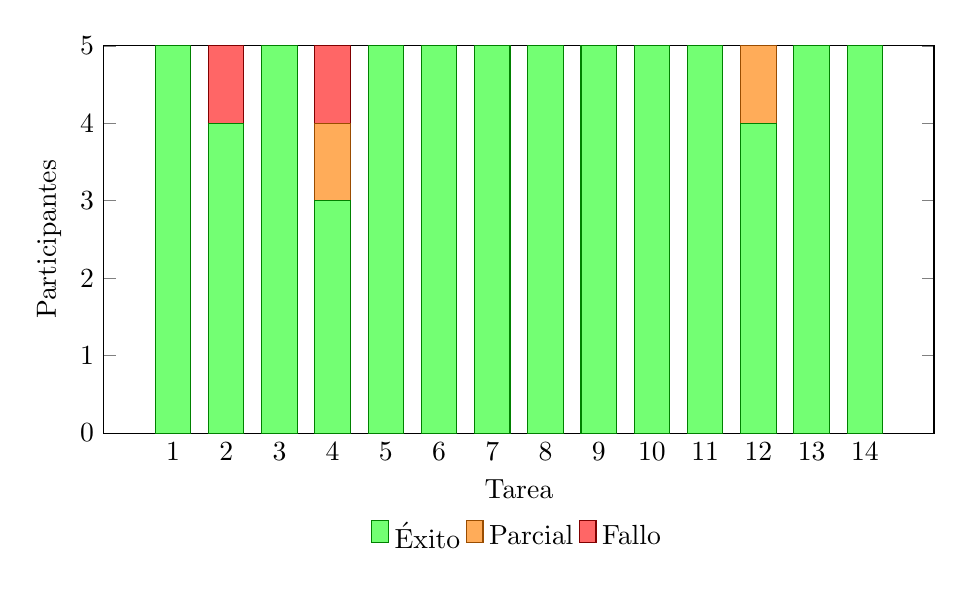
\begin{tikzpicture}
\begin{axis}[
    ybar stacked,
    bar width=0.45cm,
    width=\textwidth,
    height=6.5cm,
    xlabel={Tarea},
    ylabel={Participantes},
    ymin=0, ymax=5,
    ytick={0,1,2,3,4,5},
    xtick={1,2,3,4,5,6,7,8,9,10,11,12,13,14},
    legend style={at={(0.5,-0.20)},anchor=north,legend columns=3,draw=none},
    legend cell align={left}
]
\addplot+[fill=green!55,draw=green!50!black] coordinates {
    (1,5)(2,4)(3,5)(4,3)(5,5)(6,5)(7,5)(8,5)(9,5)(10,5)(11,5)(12,4)(13,5)(14,5)
}; \addlegendentry{Éxito}
\addplot+[fill=orange!65,draw=orange!60!black] coordinates {
    (1,0)(2,0)(3,0)(4,1)(5,0)(6,0)(7,0)(8,0)(9,0)(10,0)(11,0)(12,1)(13,0)(14,0)
}; \addlegendentry{Parcial}
\addplot+[fill=red!60,draw=red!50!black] coordinates {
    (1,0)(2,1)(3,0)(4,1)(5,0)(6,0)(7,0)(8,0)(9,0)(10,0)(11,0)(12,0)(13,0)(14,0)
}; \addlegendentry{Fallo}
\end{axis}
\end{tikzpicture}
\caption[Distribución de la completitud por tarea]{Distribución de la completitud por tarea. Las situaciones que no resultaron en éxito
limpio se concentran en T4 (filtros de exclusión, dos parciales/fallos), T12 (reordenación
de paneles, un parcial) y T2 (filtrar por metadatos, un fallo derivado de una mala
interpretación inicial de la tarea).}
\label{fig:tasaExitoTareas}
\end{figure}

La concentración de incidencias en T4 y T12 anticipa los hallazgos cualitativos discutidos
más adelante: el paso del modo \textit{Include} a \textit{Exclude} es el punto donde más
participantes tropiezan, y el comportamiento del arrastre de paneles cuando hay
\textit{scroll} vertical es el segundo foco de fricción.

\subsection{Tiempo por tarea}

El cuadro~\ref{tab:tiemposTareas} resume los tiempos por tarea en segundos. Empleamos la
mediana como medida central (más robusta que la media para muestras pequeñas) y reportamos
el mínimo y el máximo para revelar la dispersión.

\begin{table}[H]
\centering
\small
\begin{tabular}{c l r r r r}
\hline
\textbf{T} & \textbf{Tarea}                       & \textbf{Mediana} & \textbf{Mín.} & \textbf{Máx.} & \textbf{N éxito} \\
\hline
1  & Empezar a navegar                            & 15  & 5   & 21  & 5/5 \\
2  & Filtrar por metadatos                        & 16  & 7   & 45  & 4/5 \\
3  & Combinar varios filtros                      & 30  & 11  & 77  & 5/5 \\
4  & Filtros de exclusión                         & 73  & 49  & 148 & 3/5 \\
5  & Filtros de referencia                        & 5   & 2   & 55  & 5/5 \\
6  & Quitar filtros                               & 27  & 11  & 35  & 5/5 \\
7  & Seguir un \textit{link}                      & 7   & 2   & 110 & 5/5 \\
8  & Ver el historial de navegación               & 19  & 5   & 30  & 5/5 \\
9  & Volver atrás un paso                         & 6   & 2   & 25  & 5/5 \\
10 & Ver el detalle de una entidad                & 20  & 7   & 65  & 5/5 \\
11 & Guardar en \textit{Union} y cambiar          & 44  & 30  & 75  & 5/5 \\
12 & Reordenar paneles                            & 33  & 6   & 45  & 4/5 \\
13 & Cambiar de colección (sin \textit{Union})    & 13  & 5   & 45  & 5/5 \\
14 & Salir del modo navegación                    & 10  & 3   & 10  & 5/5 \\
\hline
\end{tabular}
\caption[Tiempos y éxitos por tarea]{Tiempos por tarea (segundos) y número de éxitos limpios sobre cinco intentos. Los
tiempos elevados en T4 reflejan tanto la dificultad intrínseca como la asistencia ligera
que requirieron varios participantes.}
\label{tab:tiemposTareas}
\end{table}

Tres patrones merecen comentario explícito. Primero, T4 (filtros de exclusión) destaca con
una mediana de 73~segundos, casi triple que la siguiente tarea más costosa, y un máximo de
148~segundos cercano al límite de tiempo. Segundo, T7 (seguir un \textit{link}) presenta
una varianza atípica (mediana de 7~segundos pero máximo de 110): los dos participantes que
tardaron más no encontraron el panel de \textit{links} de inmediato porque éste quedaba por
debajo del primer pliegue de la pantalla, lo cual conecta con un hallazgo cualitativo
recurrente sobre el tamaño de la interfaz. Tercero, las tareas que ejercen el modelo de
navegación recuperable (T9 \textit{Go Back}, T13 \textit{Change} y T14 \textit{Exit})
resultan rápidas y consistentes, lo que sugiere que la diferenciación visual ámbar/azul/gris
de la barra superior funciona en términos de eficiencia, aunque más adelante veremos que la
diferenciación conceptual entre \textit{Go Back} y \textit{Restore} sigue siendo borrosa
para algunos participantes.

\subsection{Facilidad percibida (SEQ)}

Para cada tarea, los participantes respondieron a la pregunta \textit{Single Ease Question}
en escala de 1 (muy difícil) a 7 (muy fácil). El gráfico~\ref{fig:seqTareas} muestra la
media por tarea. Los valores quedan, en general, por encima de 6 (es decir, en el rango
positivo), con la única excepción notable de T4, que cae a 3{,}4 y se sitúa por debajo del
umbral de 4 que suele considerarse como frontera entre tareas percibidas como aceptables y
problemáticas. T11 (\textit{Union}) y T12 (reordenar paneles) ocupan una zona intermedia
en torno a 5, coherente con la fricción detectada en sus tiempos.

\begin{figure}[H]
\centering
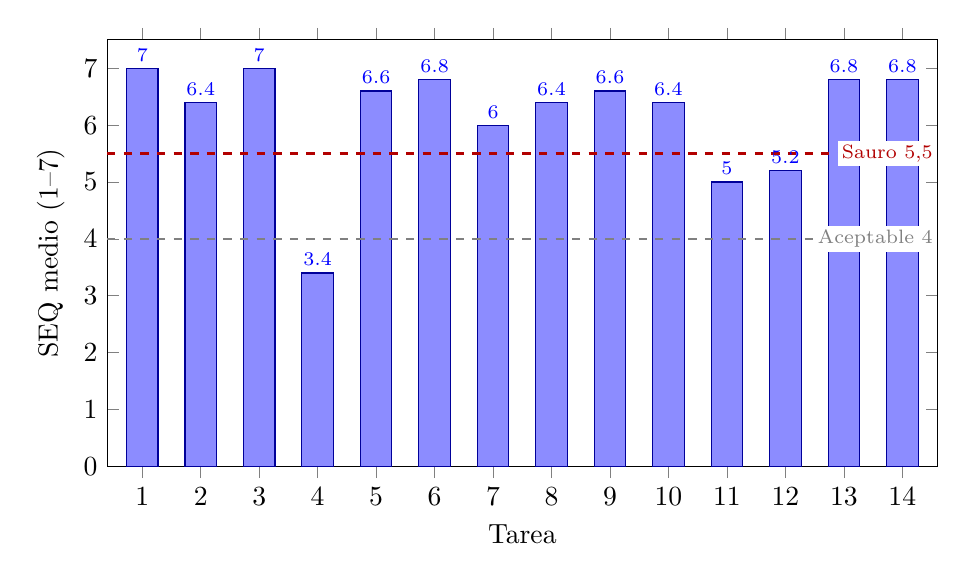
\begin{tikzpicture}
\begin{axis}[
    ybar,
    bar width=0.4cm,
    width=\textwidth,
    height=7cm,
    xlabel={Tarea},
    ylabel={SEQ medio (1--7)},
    ymin=0, ymax=7.5,
    ytick={0,1,2,3,4,5,6,7},
    xtick={1,2,3,4,5,6,7,8,9,10,11,12,13,14},
    xmin=0.4, xmax=14.6,
    enlarge x limits=false,
    nodes near coords,
    nodes near coords align={vertical},
    every node near coord/.append style={font=\scriptsize,yshift=-1pt}
]
\addplot+[fill=blue!45,draw=blue!60!black] coordinates {
    (1,7.0)(2,6.4)(3,7.0)(4,3.4)(5,6.6)(6,6.8)(7,6.0)(8,6.4)(9,6.6)(10,6.4)(11,5.0)(12,5.2)(13,6.8)(14,6.8)
};
\draw[red!70!black, dashed, thick] (axis cs:0.4,5.5) -- (axis cs:14.6,5.5);
\draw[gray, dashed, thick]         (axis cs:0.4,4.0) -- (axis cs:14.6,4.0);
\node[red!70!black, font=\scriptsize, fill=white, inner sep=1.5pt, anchor=east]
    at (axis cs:14.6,5.5) {Sauro 5{,}5};
\node[gray, font=\scriptsize, fill=white, inner sep=1.5pt, anchor=east]
    at (axis cs:14.6,4.0) {Aceptable 4};
\end{axis}
\end{tikzpicture}
\caption[Facilidad percibida (SEQ) por tarea]{Facilidad percibida (SEQ) media por tarea. Las líneas discontinuas marcan el umbral
de aceptación clásico (SEQ~$\geq$~4) y la referencia de Sauro para tareas «fáciles»
(SEQ~$\geq$~5{,}5). Sólo T4 cae por debajo del primer umbral.}
\label{fig:seqTareas}
\end{figure}

\subsection{Satisfacción global (SUS)}

Las puntuaciones SUS individuales y la media del grupo aparecen en el
gráfico~\ref{fig:susParticipantes}. Las cinco puntuaciones quedan por encima del umbral
clásico de 68 que separa los sistemas «aceptables» de los que no lo son, y cuatro
de las cinco superan el umbral de 80 que se asocia con sistemas «excelentes». La
media del grupo, \textbf{85}, se sitúa en el primer cuartil de la distribución de
referencia de Sauro y Lewis, lo que constituye uno de los resultados más sólidos del
estudio.

\begin{figure}[H]
\centering
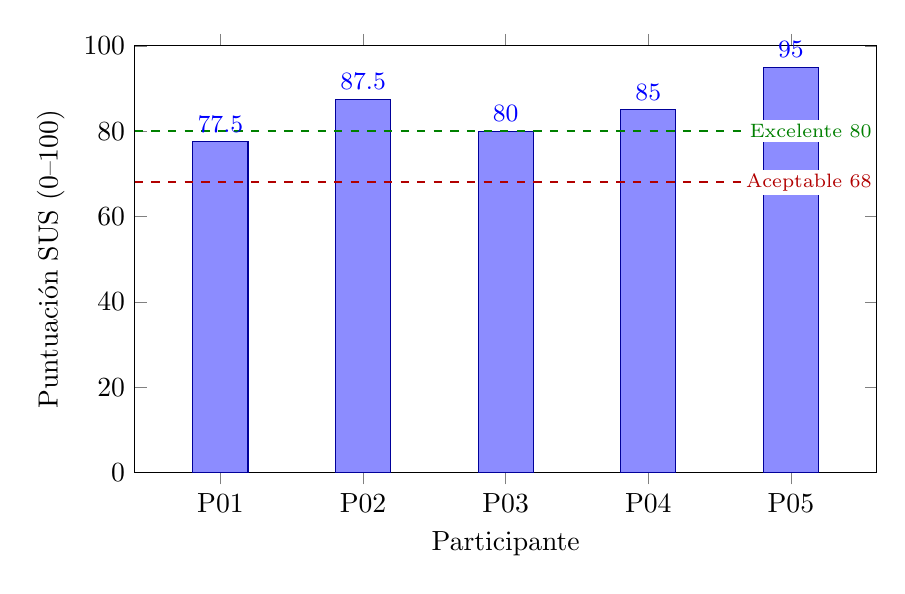
\begin{tikzpicture}
\begin{axis}[
    ybar,
    bar width=0.7cm,
    width=11cm,
    height=7cm,
    xlabel={Participante},
    ylabel={Puntuación SUS (0--100)},
    ymin=0, ymax=100,
    ytick={0,20,40,60,80,100},
    symbolic x coords={P01,P02,P03,P04,P05},
    xtick=data,
    nodes near coords,
    every node near coord/.append style={font=\small},
    enlarge x limits=0.15
]
\addplot+[fill=blue!45,draw=blue!60!black] coordinates {
    (P01,77.5) (P02,87.5) (P03,80) (P04,85) (P05,95)
};
% Horizontal reference lines spanning the full plot width (use rel axis
% cs for the X bounds so they sit edge-to-edge regardless of bar layout).
\draw[red!70!black, dashed, thick]
    ({rel axis cs:0,0} |- {axis cs:P01,68}) --
    ({rel axis cs:1,0} |- {axis cs:P01,68});
\draw[green!50!black, dashed, thick]
    ({rel axis cs:0,0} |- {axis cs:P01,80}) --
    ({rel axis cs:1,0} |- {axis cs:P01,80});
\node[red!70!black, font=\scriptsize, fill=white, inner sep=1.5pt, anchor=east]
    at ({rel axis cs:1,0} |- {axis cs:P01,68}) {Aceptable 68};
\node[green!50!black, font=\scriptsize, fill=white, inner sep=1.5pt, anchor=east]
    at ({rel axis cs:1,0} |- {axis cs:P01,80}) {Excelente 80};
\end{axis}
\end{tikzpicture}
\caption[Puntuación SUS por participante]{Puntuación SUS por participante. La media del grupo es 85, con todos los valores
por encima del umbral de aceptación (68) y cuatro de cinco por encima del umbral de
excelencia (80).}
\label{fig:susParticipantes}
\end{figure}

\section{Hallazgos cualitativos y problemas detectados}
\label{sec:hallazgosCualitativos}

El cruce de las observaciones del facilitador, los comentarios espontáneos en
\textit{think-aloud} y las respuestas a las preguntas abiertas de cierre permite agrupar
los problemas detectados en cinco familias, ordenadas en el cuadro~\ref{tab:incidenciasNielsen}
por gravedad estimada según la escala de Nielsen y por frecuencia de aparición.

\begin{table}[H]
\centering
\small
\begin{tabularx}{\textwidth}{X c c c}
\hline
\textbf{Problema}                                                  & \textbf{Gravedad} & \textbf{Frecuencia} & \textbf{Tareas} \\
\hline
Toggle \textit{Include}/\textit{Exclude} poco descubrible          & 3 (mayor)   & 5/5 & T4 \\
Arrastre de paneles sin \textit{auto-scroll} cuando hay desbordamiento & 2 (menor) & 3/5 & T12 \\
Distinción \textit{Restore} vs \textit{Go Back}                    & 2 (menor)   & 2/5 & T9, T13 \\
Visibilidad de los paneles inferiores (\textit{links}, entidades)  & 2 (menor)   & 2/5 & T7, T10 \\
Concepto de \textit{Union Set} sin pistas                          & 1 (cosmético) & 2/5 & T11 \\
\hline
\end{tabularx}
\caption[Catálogo de incidencias detectadas]{Catálogo de incidencias detectadas, ordenadas por gravedad. La gravedad sigue
la escala clásica de Nielsen (0 = sin problema, 1 = cosmético, 2 = menor, 3 = mayor,
4 = catastrófico) y la frecuencia indica sobre cuántos de los cinco participantes apareció.}
\label{tab:incidenciasNielsen}
\end{table}

El \textbf{toggle de inclusión y exclusión} es el problema más nítido del estudio. Los cinco
participantes intentaron, en algún momento de T4, cambiar el sentido del filtro pulsando
directamente sobre la etiqueta verde con «+», esperando que mutase a la versión roja
con «$-$». El control real (un botón segmentado en la cabecera del panel de Filtros)
sólo se descubría tras varios segundos de exploración o, en el caso de P05, no se descubría
en absoluto. Las tres respuestas a la pregunta de cierre sobre lo más confuso del sistema
mencionan literalmente este punto, y P01 lo expresa con claridad: «piensa que sería más
intuitivo poder dar click al "+" de tal manera que se convierta en un "-"». Adicionalmente,
la previsualización por \textit{hover} introducida para anticipar la acción del clic generó
confusión: al pasar el ratón el texto cambiaba pero, al hacer clic, el ratón seguía sobre
el botón y el cambio aparente de estado se confundía con la previsualización en curso. La
combinación de un toggle separado del filtro y una previsualización ambigua acumula dos
fuentes de fricción sobre la misma acción.

El \textbf{arrastre de paneles} (T12) funcionó correctamente cuando el panel de origen y
el de destino cabían en la pantalla, pero falló sistemáticamente cuando el destino estaba
fuera del \textit{viewport}: tres participantes intentaron arrastrar un panel hacia arriba
sin que la página realizase \textit{auto-scroll}, lo que rompió la metáfora de manipulación
directa. Dos de ellos consiguieron completar la tarea por una vía alternativa, pero P01
quedó en parcial. Es un fallo de implementación del \textit{drag-and-drop} más que un fallo
de diseño, pero el efecto sobre la percepción es desproporcionado.

La \textbf{distinción entre \textit{Restore} y \textit{Go Back}} sigue siendo problemática
para una minoría significativa. Aunque la diferenciación visual de la barra superior
(ámbar / azul / gris) sí se percibe como una pista de uso, el modelo conceptual no se
deriva sin pistas: P01 y P05 invierten el papel de los dos botones cuando se les pide
explicarlos al final de la sesión. P02 y P03 los explican correctamente, lo que sugiere
que el problema afecta sobre todo a participantes con menor familiaridad con interfaces
de exploración.

La \textbf{visibilidad de los paneles inferiores} se manifestó como una serie de pequeñas
fricciones en T7 y T10. Dos participantes (P01, P02) no descubrieron de inmediato la
existencia del panel de \textit{links} ni del de entidades porque ambos quedaban por debajo
del primer pliegue de la pantalla en su configuración inicial, e intentaron resolver la
tarea con los controles visibles. P02 sintetizó el problema durante la sesión: «siente
que la interfaz es un poco grande y hay que ir moviéndose por ella».

El \textbf{concepto de \textit{Union Set}} es el caso más matizado. Cuatro de cinco
participantes lo entendieron en el momento del uso (T11 se completa con éxito en los
cinco casos), pero al pedirles que lo explicasen con sus propias palabras al final de la
sesión, dos no consiguieron articular su semántica más allá de «se han guardado cosas».
Esto sugiere que la interfaz comunica bien la operación inmediata pero no necesariamente
el modelo subyacente. P02, con formación en bases de datos, lo asoció directamente con la
unión matemática.

Las preguntas abiertas dejaron también un conjunto de \textbf{solicitudes de funcionalidad}
recurrentes que conviene registrar aunque excedan el alcance del trabajo: búsqueda por
texto sobre los nombres de los metadatos y sobre las entidades (P01), previsualizaciones
ricas con miniaturas en el panel de entidades (P01, P04), navegación anidada de entidades
dentro de entidades (P04) y una sección de ayuda contextual (P03). Algunas de estas se
recogen como líneas de trabajo futuro en el capítulo~\ref{cap:conclusiones}.

\section{Iteraciones de la interfaz derivadas de la evaluación}
\label{sec:iteracionesUI}

Cinco direcciones concretas de modificación se desprenden del catálogo anterior. La primera,
de mayor prioridad, consiste en \textbf{rediseñar la interacción de inclusión y exclusión}.
La hipótesis a explorar, sugerida por varios participantes, es que la propia etiqueta del
filtro activo se comporte como un toggle: pulsar sobre el «+» verde lo convertiría en
«$-$» rojo y viceversa, de manera que el control segmentado actual quede como un valor
por defecto al añadir filtros nuevos pero no como el único punto de cambio. La previsualización
por \textit{hover} debería desactivarse o convertirse en un \textit{tooltip} explícito para
evitar la confusión observada.

La segunda dirección es \textbf{implementar \textit{auto-scroll} durante el arrastre de paneles}:
cuando el cursor se acerca al borde superior o inferior del \textit{viewport} mientras se
arrastra un panel, la página debe desplazarse en esa dirección. Es un cambio puramente técnico
en la lógica de \textit{drag-and-drop} pero recupera la metáfora de manipulación directa que
los participantes esperan.

La tercera consiste en \textbf{reforzar la diferenciación entre \textit{Restore} y \textit{Go Back}},
ya sea mediante etiquetas más explícitas (por ejemplo, «Deshacer último link» y
«Restaurar estado guardado»), un \textit{tooltip} la primera vez que el usuario pasa
sobre cada botón, o ambos. La diferenciación visual actual ayuda en eficiencia pero no
construye el modelo conceptual.

La cuarta es \textbf{mejorar la visibilidad de los paneles inferiores}. Caben varias
estrategias: compactar la altura inicial del panel de Filtros para que el panel de
entidades quede dentro del primer pliegue; introducir un indicador visual de «hay más
contenido más abajo»; o reorganizar el orden por defecto de manera que las áreas de
acción más frecuente queden primero. La elección entre estas opciones es a su vez
candidata a una nueva ronda de evaluación.

La quinta y última es \textbf{aclarar el concepto de \textit{Union Set}} mediante una
introducción contextual la primera vez que el usuario pulsa «+ Add current» (un
\textit{tooltip} explicativo, una pequeña anotación en el panel cuando está vacío, o un
recorrido guiado opcional al inicio de la primera sesión). El comportamiento del sistema
es correcto; lo que falta es comunicación.

\section{Casos de uso validados}
\label{sec:casosDeUsoValidados}

El cuadro~\ref{tab:casosDeUsoValidados} resume el estado de validación de cada caso de uso
del sistema cruzando las tareas de la evaluación con su tasa de éxito y SEQ medio. Sirve
como vista compacta del veredicto del estudio: la mayoría de los casos de uso quedan
validados sin reservas; los dos casos asociados a la fricción detectada (filtros de
exclusión y operaciones de conjunto / personalización del espacio) se consideran validados
con observaciones que deberán abordarse en la siguiente iteración.

\begin{table}[H]
\centering
\small
\begin{tabularx}{\textwidth}{X c c c c}
\hline
\textbf{Caso de uso}                                  & \textbf{Tareas}   & \textbf{Éxito} & \textbf{SEQ} & \textbf{Veredicto} \\
\hline
Selección de dataset y colección                      & T1                & 5/5 & 7{,}0 & Validado \\
Filtrado por metadatos                                & T2, T3            & 9/10 & 6{,}7 & Validado \\
Filtrado por exclusión                                & T4                & 3/5 & 3{,}4 & Validado con observaciones \\
Filtros de referencia                                 & T5                & 5/5 & 6{,}6 & Validado \\
Gestión de filtros activos                            & T6                & 5/5 & 6{,}8 & Validado \\
Navegación transversal por \textit{links}             & T7, T9            & 10/10 & 6{,}3 & Validado \\
Historial visual de la navegación                     & T8                & 5/5 & 6{,}4 & Validado \\
Inspección de entidad (modal de detalle)              & T10               & 5/5 & 6{,}4 & Validado \\
Operaciones de conjunto (\textit{Union})              & T11               & 5/5 & 5{,}0 & Validado con observaciones \\
Personalización del espacio (reordenar paneles)       & T12               & 4/5 & 5{,}2 & Validado con observaciones \\
Cambios destructivos con confirmación                 & T13, T14          & 10/10 & 6{,}8 & Validado \\
\hline
\end{tabularx}
\caption[Resumen de casos de uso validados]{Resumen de casos de uso validados. La columna \textit{Veredicto} distingue entre
casos validados sin reservas (todos los participantes los completaron con SEQ medio
$\geq$~6) y casos validados con observaciones, donde la operativa funciona pero la
evaluación detectó fricción que se aborda en la sección~\ref{sec:iteracionesUI}.}
\label{tab:casosDeUsoValidados}
\end{table}

\section{Limitaciones del estudio}
\label{sec:limitacionesEstudio}

El estudio presentado debe interpretarse dentro de varios límites bien delimitados. El más
evidente es el \textbf{tamaño muestral}: cinco participantes son suficientes para detectar la
mayoría de los problemas observables siguiendo la heurística clásica de Nielsen, pero no
permiten sostener afirmaciones cuantitativas con valor estadístico inferencial. Las medias
de SUS y SEQ que se reportan describen el grupo concreto evaluado y deben leerse como
indicadores cualitativos antes que como estimaciones de una población.

El \textbf{perfil de los participantes}, aunque diversificado en edad, ocupación y experiencia
previa, no es representativo de los usuarios reales del sistema en producción, fundamentalmente
porque tales usuarios no existen aún: el sistema se ha evaluado sobre catálogos de prueba y
no sobre un despliegue real con población definida. Esto introduce un sesgo inevitable, ya
que los participantes interpretan las tareas en abstracto en lugar de hacerlo movidos por
una necesidad propia de exploración.

El \textbf{dominio de la evaluación} fue el catálogo TMDB, escogido por su familiaridad
universal y por reducir el coste cognitivo de comprender los datos. La validación con DBLP,
de naturaleza estructural distinta, se quedó en el plano funcional descrito en la
sección~\ref{sec:validacionFuncional} y no se trasladó a la evaluación con usuarios. Es
razonable suponer que parte de los hallazgos de usabilidad serían comunes a ambos dominios,
pero también que la familiaridad del usuario con películas frente a publicaciones científicas
modula las observaciones.

Por último, se trata de un estudio \textbf{sin grupo de control}: no se ha comparado el
rendimiento de los participantes con el que tendrían sobre una herramienta alternativa
(búsqueda directa, filtrado clásico, etcétera), de manera que las afirmaciones sobre la
adecuación del sistema deben entenderse en términos absolutos y no comparativos. Una
evaluación comparada con una segunda interfaz constituye, junto al despliegue real con
usuarios identificados, una de las extensiones naturales del trabajo, recogida también
entre las líneas futuras del capítulo~\ref{cap:conclusiones}.
